\documentclass[12pt]{article}

\setlength{\topmargin}{-.75in} \addtolength{\textheight}{2.00in}
\setlength{\oddsidemargin}{.00in} \addtolength{\textwidth}{.75in}

\usepackage{amsmath,color,graphicx,array,multirow,rotating, enumerate}
\usepackage{type1cm}
\usepackage{eso-pic}
\usepackage[hmargin=2cm,vmargin=1.3cm]{geometry}
\usepackage{mathabx}
\usepackage[rflt]{/Users/jgates/desktop/latex/floatflt}
\usepackage[table]{xcolor}
\nofiles

\def\Tab#1{\tabular[t]{>{\rule[-1ex]{0pt}{3ex}}c}#1\endtabular}
\newcolumntype{C}{@{}c@{}}

\pagestyle{empty}
\newcounter{ProbNum}
\setlength{\parindent}{0in}

% Watermark: graph paper
\newcommand\BackgroundPic{
\put(0,0){
\parbox[b][\paperheight]{\paperwidth}{%
\vfill
\centering

\includegraphics[width=\paperwidth,height=\paperheight,keepaspectratio]{/Users/jgates/desktop/latex/pics/plain.pdf}%
\vfill
}}}

%Diagram box command [v space][content]
\newcommand{\diagrambox}[2][40 mm]{
\framebox{\parbox{175 mm}{#2 \hfill \\ \vspace{#1}}}

\bigskip
}

% MakeList: [example number] [content]
\newcommand{\MakeList}[2]{
\begin{enumerate}[#1] \itemsep1pt \parskip0pt \parsep0pt  

#2
\end{enumerate}
}

\begin{document}



{\Large Problems tagged with standards:}CAPMA
\bigskip 
% Number 350
% CAPMA Algebra Units
% Car slowing up hill
% JG

% Watermark
\AddToShipoutPicture*{\BackgroundPic}

\addtocounter {ProbNum} {1}

%\begin{floatingfigure}[r]{.3\textwidth}
%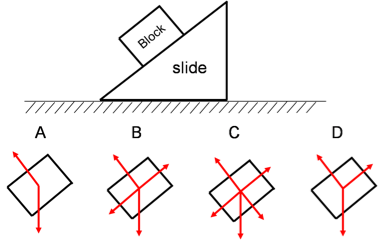
\includegraphics[scale=.4]{/Users/jgates/desktop/latex/pics/incline3.png}
%\end{floatingfigure}
 
{\bf \Large{350.}} A car that is moving ${30~\tfrac{m}{s}}$ runs out of gas while driving up a hill.  The car comes to a stop 150 meters further up the hill than the point at which it ran out of gas. 

\begin{center}
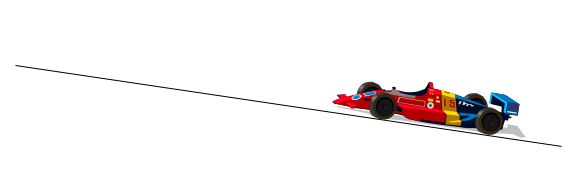
\includegraphics[scale=.6]{/Users/jgates/desktop/latex/pics/caruphill.png}
\end{center}

\bigskip  How long, after running out of gas, did it take for the car to come to a stop?  Also describe, in words, the direction of the acceleration. Draw a kinematics diagram as part of your solution.


\bigskip \vspace{6mm}% Number 370
% CAPMA Algebra Units
% Cannon shot straight up - how much time? Graphical
% JG

% Watermark
\AddToShipoutPicture*{\BackgroundPic}

\addtocounter {ProbNum} {1}

%\begin{floatingfigure}[r]{.15\textwidth}
%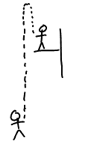
\includegraphics[scale=.8]{/Users/jgates/desktop/latex/pics/tokentoss.png}
%\end{floatingfigure}
 
{\bf \Large{370.}} A cannon is shot straight up into the air. The cannonball leaves the cannon moving ${45~\tfrac{m}{s}}$.  

\bigskip  After how much time in the air will it have a speed of ${20~\tfrac{m}{s}}$? 

%\begin{center}
%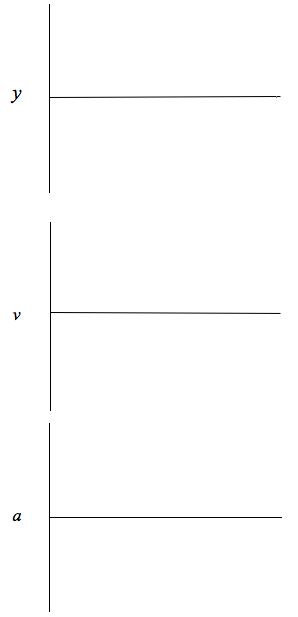
\includegraphics[scale=.85]{/Users/jgates/desktop/latex/pics/blankyvagraphstack.png}
%\end{center}


\bigskip \vspace{6mm}% Number 372
% CAPMA Algebra Units
% Cannon shot straight up - how much time? Algebraic
% JG

% Watermark
\AddToShipoutPicture*{\BackgroundPic}

\addtocounter {ProbNum} {1}

%\begin{floatingfigure}[r]{.15\textwidth}
%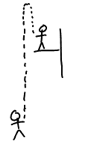
\includegraphics[scale=.8]{/Users/jgates/desktop/latex/pics/tokentoss.png}
%\end{floatingfigure}
 
{\bf \Large{372.}} A cannon is shot straight up into the air. The cannonball leaves the cannon moving ${45~\tfrac{m}{s}}$.  

\bigskip  After how much time in the air will it have a speed of ${20~\tfrac{m}{s}}$? Use algebraic problem-solving.

%\begin{center}
%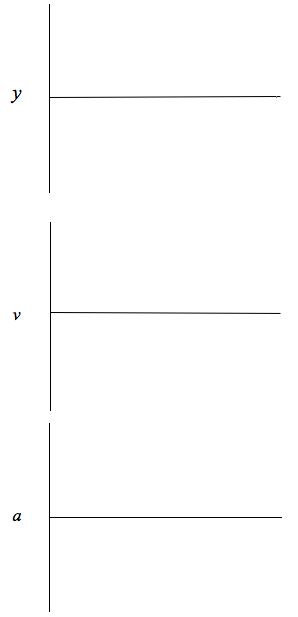
\includegraphics[scale=.85]{/Users/jgates/desktop/latex/pics/blankyvagraphstack.png}
%\end{center}


\bigskip \vspace{6mm}% Number 391
% CAPMA Algebra Units
% Meteor chunk slowdown; algebraic version
% JG

% Watermark
\AddToShipoutPicture*{\BackgroundPic}

\addtocounter {ProbNum} {1}

%\begin{floatingfigure}[r]{.15\textwidth}
%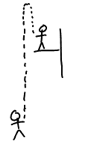
\includegraphics[scale=.8]{/Users/jgates/desktop/latex/pics/tokentoss.png}
%\end{floatingfigure}
 
{\bf \Large{391.}} A rock fragment is traveling ${640~\tfrac{m}{s}}$  when it is knocked off of a falling meteor. It has slowed to ${590~\tfrac{m}{s}}$  after .6 seconds.  Assume a constant acceleration. 

\bigskip
How far will it have gone after 2 seconds? Use algebraic problem-solving.

%\begin{center}
%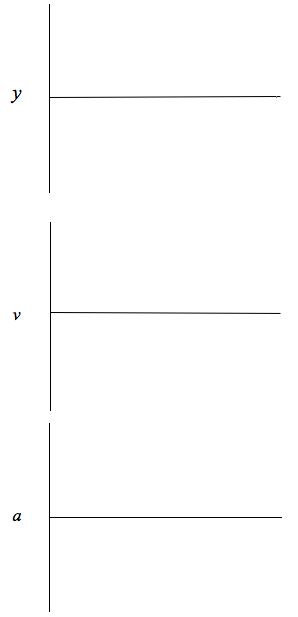
\includegraphics[scale=.85]{/Users/jgates/desktop/latex/pics/blankyvagraphstack.png}
%\end{center}


\bigskip \vspace{6mm}% Number 500
% CAPMA CVPMA 
% Stoplight stopping
% KO

% Watermark
\AddToShipoutPicture*{\BackgroundPic}

\addtocounter {ProbNum} {1}

%\begin{floatingfigure}[r]{.33\textwidth}
%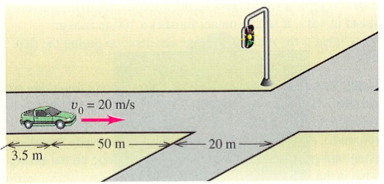
\includegraphics[scale=.6]{/Users/jgates/desktop/latex/pics/redlight}
%\end{floatingfigure}
 
{\bf \Large{500.}} A car 3.5 m in length and traveling at a constant speed of ${20~\tfrac{m}{s}}$ is approaching an intersection. The width of the intersection is 20 m. The light turns yellow when the front of the car is 50 m from the beginning of the intersection. If the driver steps on the brake, the car will slow at a rate of ${4.2~\tfrac{m}{s}}$ per second. If the driver instead steps on the gas pedal, the car will accelerate at ${1.5~\tfrac{m}{s^2}}$. The light will be yellow for 3 seconds. Ignore the reaction time of the driver. 

\bigskip
To avoid being in the intersection while the light is red, should the driver hit the brake pedal or the gas pedal? Justify your answer with some pretty physics.

\hfill 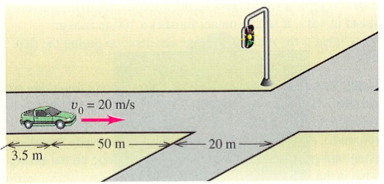
\includegraphics[scale=.85]{/Users/jgates/desktop/latex/pics/redlight.png}


\bigskip \vspace{6mm}% Number 530
% UFPM SFriction KFriction Algebra Units CAPMA
% Sliding crate on truck bed - friction
% KO

% Watermark
\AddToShipoutPicture*{\BackgroundPic}

\addtocounter {ProbNum} {1}

%\begin{floatingfigure}[r]{.45\textwidth}
%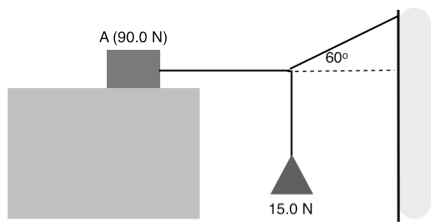
\includegraphics[scale=.6]{/Users/jgates/desktop/latex/pics/static1}
%\end{floatingfigure}
 
{\bf \Large{530.}} A 20 kg box rests on the flat floor of a truck. The coefficients of friction between the box and floor are ${\mu_s=.15}$ and ${\mu_k=.1}$. The truck stops gently at a stop sign and then starts to move with a constant acceleration. The box is 2.2 m from the rear of the truck when the truck starts.

\bigskip
What is the maximum possible acceleration that the truck may have if the box is not to slide?

\bigskip Suppose that the acceleration of the truck is instead ${2.1~\tfrac{m}{s^2}}$. How much time elapses before the box falls off the rear of the truck? 

\bigskip How far does the truck travel in this time?

%\hfill 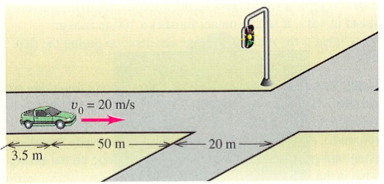
\includegraphics[scale=.85]{/Users/jgates/desktop/latex/pics/redlight.png}


\bigskip \vspace{6mm}% Number 540
% UFPM Vectors Algebra Units CAPMA CVPMA
% Wagon rolling down hill
% KO/JG

% Watermark
\AddToShipoutPicture*{\BackgroundPic}

\addtocounter {ProbNum} {1}

%\begin{floatingfigure}[r]{.45\textwidth}
%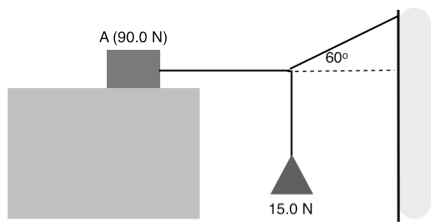
\includegraphics[scale=.6]{/Users/jgates/desktop/latex/pics/static1}
%\end{floatingfigure}
 
{\bf \Large{540.}} A wagon with two boxes of gold (total mass 300 kg) is cut loose from the horses by an outlaw when the wagon is at rest 50 m up a 6 degree slope. The outlaw plans to have the wagon roll down the slope and across the level ground, and then fall into a canyon where his confederates wait. 

\bigskip
Find the speed of the wagon when it reaches the flat ground. Note that it starts from rest at the top of the incline and that the wagon rolls with negligible friction.

\bigskip 
\bigskip If another bandit standing at the end of the slope requires twenty seconds to grab the gold, how far must the edge of the cliff be from the end of the slope, in order to make this double-heist successful?

%\hfill 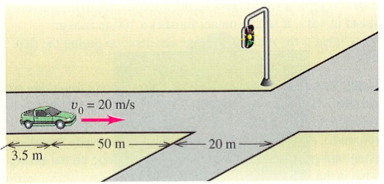
\includegraphics[scale=.85]{/Users/jgates/desktop/latex/pics/redlight.png}


\bigskip \vspace{6mm}% Number 550
% UFPM SFriction Algebra Units CAPMA KFriction
% Block held up to vertical cart by acceleration/friction
% KO/JG

% Watermark
\AddToShipoutPicture*{\BackgroundPic}

\addtocounter {ProbNum} {1}

\begin{floatingfigure}[r]{.2\textwidth}
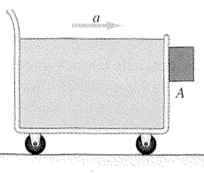
\includegraphics[scale=.6]{/Users/jgates/desktop/latex/pics/cartstatic}
\end{floatingfigure}
 
{\bf \Large{550.}} The cart accelerates to the right, keeping block A from sliding down. The coefficient of static friction between the block and the cart is .8, and the coefficient of kinetic friction is .5. The block is 1.2 meters above the ground.

\bigskip
What minimum acceleration must the cart have in order that block A does not fall? 

\bigskip If the acceleration of the cart were only half that value, how long would it take for the block to hit the ground?
%\hfill 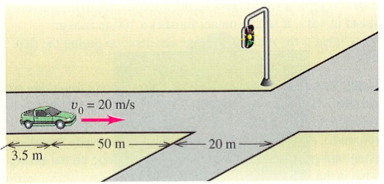
\includegraphics[scale=.85]{/Users/jgates/desktop/latex/pics/redlight.png}

\bigskip \bigskip \vspace{6mm}% Number 560
% UFPM  Algebra Units CAPMA 
% Airbag Stop
% KO/JG

% Watermark
\AddToShipoutPicture*{\BackgroundPic}

\addtocounter {ProbNum} {1}

%\begin{floatingfigure}[r]{.2\textwidth}
%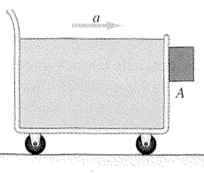
\includegraphics[scale=.6]{/Users/jgates/desktop/latex/pics/cartstatic}
%\end{floatingfigure}
 
{\bf \Large{560.}} The human body can survive a negative acceleration trauma incident (sudden stop) if the magnitude of the acceleration is less than ${250~\tfrac{m}{s^2}}$ (approximately 25g), as a rule of thumb. Suppose that you are in an automobile accident with an initial speed of ${105~\tfrac{km}{hr}}$ (65 mph) and are stopped by an airbag that inflates from the dashboard. 

\bigskip
Over what distance must the airbag stop you for you to survive the crash?

\bigskip How much time will it take for the airbag to stop you?

\bigskip What average force will be exerted on you by the airbag?

\bigskip \vspace{6mm}% Number 590
% UFPM  Inclines CAPMA CAPMG Algebra Units 
% Cart sliding up incline
% JG

% Watermark
\AddToShipoutPicture*{\BackgroundPic}

\addtocounter {ProbNum} {1}

%\begin{floatingfigure}[r]{.2\textwidth}
%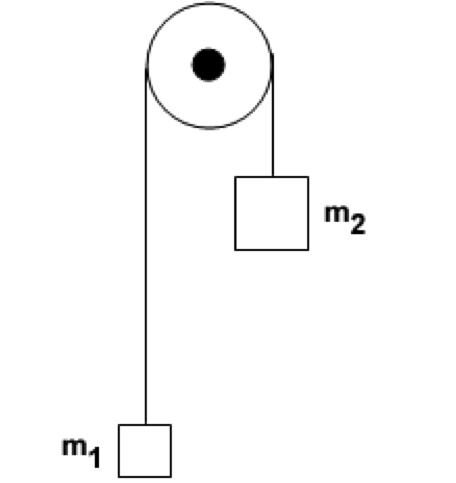
\includegraphics[scale=.8]{/Users/jgates/desktop/latex/pics/Atwood3}
%\end{floatingfigure}
 
{\bf \Large{590.}} A glider is given a quick push to start it moving up a ${7^{\circ}}$ inlined air track. The glider travels to a maximum distance of 112 cm up the track.

\bigskip
Determine the initial speed of the glider.
 
\bigskip \bigskip 
Draw a velocity graph for the glider; use the graph to determine how long the glider takes to get to that 112 cm point.
\bigskip 
Use your velocity graph to determine where the glider will be 2 seconds after it was launched.
\bigskip %\hfill 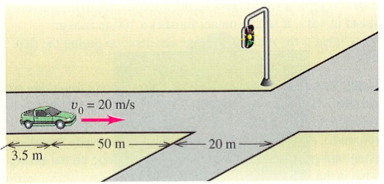
\includegraphics[scale=.85]{/Users/jgates/desktop/latex/pics/redlight.png}
\vspace{6mm}% Number 600
% CAPMA CAPMG Algebra Units 
% Overtaking - CAPM and CVPM
% JG

% Watermark
\AddToShipoutPicture*{\BackgroundPic}

\addtocounter {ProbNum} {1}

%\begin{floatingfigure}[r]{.2\textwidth}
%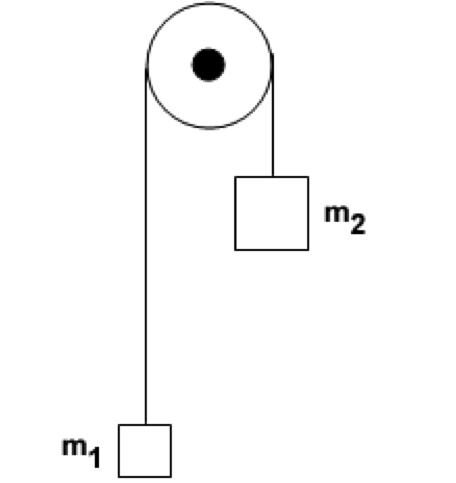
\includegraphics[scale=.8]{/Users/jgates/desktop/latex/pics/Atwood3}
%\end{floatingfigure}
 
{\bf \Large{600.}} A police car is driving towards a parked pair of criminals eating Zagnuts after pulling off a heist. The police car is moving ${40~\tfrac{m}{s}}$ and is initially .4 km away from the criminals. The criminals are going to drive away from the police car in an attempt to escape.  Assume that the crimemobile moves with a constant acceleration of ${1.8~\tfrac{m}{s^2}}$. 

\bigskip
Where will the police catch them?

\bigskip 
Draw a velocity graph for the criminals.  Use it to determine how far down they road they are when the police car passes their starting point.
\bigskip 
%\hfill 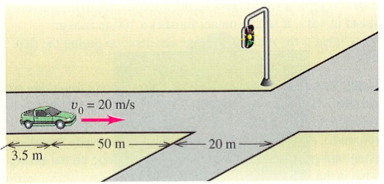
\includegraphics[scale=.85]{/Users/jgates/desktop/latex/pics/redlight.png}
\vspace{6mm}% Number 780
% CAPMA CAPMG Algebra Units 
% Rocket AP problem - graphical and algebraic
% Mostly AP/some JG

% Watermark
\AddToShipoutPicture*{\BackgroundPic}

\addtocounter {ProbNum} {1}

%\begin{floatingfigure}[r]{.44\textwidth}
%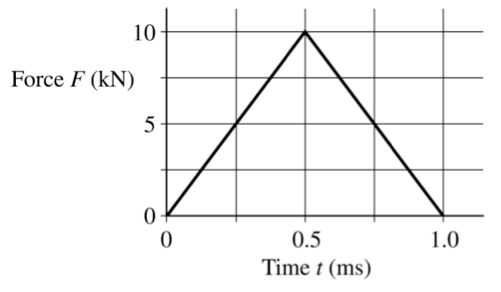
\includegraphics[scale=.5]{/Users/jgates/desktop/latex/pics/collisiongraph1}
%\end{floatingfigure}
 
{\bf \Large{780.}} A two stage rocket leaves its launch pad moving vertically with an average acceleration of ${4~\tfrac{m}{s^2}}$.  10 seconds after launch, the first stage of the rocket (now without fuel) separates from the second stage  The second stage now has an upward acceleration of ${6~\tfrac{m}{s^2}}$.  

\bigskip
How high is the rocket when the first stage separates?

\bigskip 
What will be the maximum height attained by the first stage after separation?

\bigskip 
\vspace{6mm}% Watermark
\AddToShipoutPicture*{\BackgroundPic}
Draw position, velocity, and acceleration graphs for the first and second stages' motions {\emph after separation} on the same three sets of axes (that is, have both velocity graph on one set of axes, both position graphs on another, etc.).

\bigskip 
\bigskip 
Use the graphs to determine how far apart the stages are 4 seconds after separation.

\bigskip %\hfill 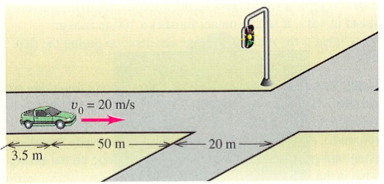
\includegraphics[scale=.85]{/Users/jgates/desktop/latex/pics/redlight.png}
\vspace{6mm}% Number 811
% CAPMA Algebra Units 
% Clay/Jax chase - algebraic
% JG

% Watermark
\AddToShipoutPicture*{\BackgroundPic}

\addtocounter {ProbNum} {1}

%\begin{floatingfigure}[r]{.44\textwidth}
%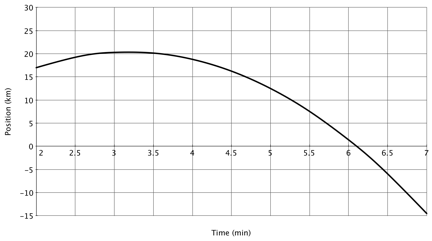
\includegraphics[scale=.5]{/Users/jgates/desktop/latex/pics/xgraph2}
%\end{floatingfigure}
 
{\bf \Large{811.}} Jax is sitting by the side of the road on his motorcycle when Clay zips by at 30 meters per second.  Jax immediately takes off in pursuit, driving with a constant acceleration.  Jax accelerates to Clay's speed within 15 seconds. \bigskip

How far behind Clay will Jax be at that moment that their speeds are equal?  Use algebraic methods. \paragraph{}
\noindent

%\begin{center}
%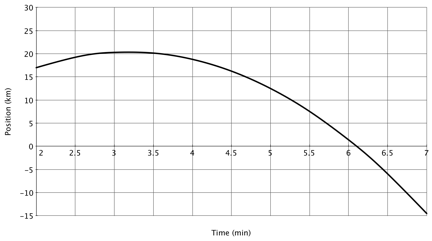
\includegraphics[scale=1]{/Users/jgates/desktop/latex/pics/xgraph2}
%\end{center}

\bigskip \vspace{6mm}% Number 812
% CAPMA Algebra Units 
% Clay/Jax chase harder - algebraic
% JG

% Watermark
\AddToShipoutPicture*{\BackgroundPic}

\addtocounter {ProbNum} {1}

%\begin{floatingfigure}[r]{.44\textwidth}
%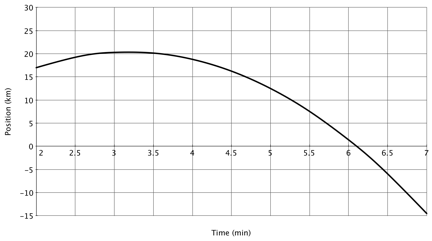
\includegraphics[scale=.5]{/Users/jgates/desktop/latex/pics/xgraph2}
%\end{floatingfigure}
 
{\bf \Large{812.}} Jax is sitting by the side of the road on his motorcycle when Clay zips by at 30 meters per second.  Jax immediately takes off in pursuit, driving with a constant acceleration.  Jax accelerates to Clay's speed within 15 seconds. \bigskip

How long will it take Jax to catch Clay?  Use algebraic methods. \paragraph{}
\noindent

%\begin{center}
%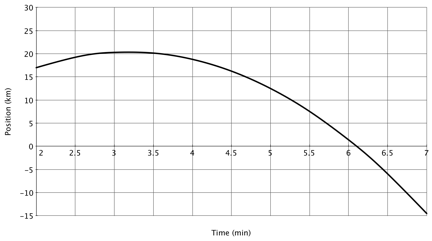
\includegraphics[scale=1]{/Users/jgates/desktop/latex/pics/xgraph2}
%\end{center}

\bigskip \vspace{6mm}% Number 820
% CAPMA Algebra Units 
% Rocket launch, freefall afterwards
% JG

% Watermark
\AddToShipoutPicture*{\BackgroundPic}

\addtocounter {ProbNum} {1}

%\begin{floatingfigure}[r]{.44\textwidth}
%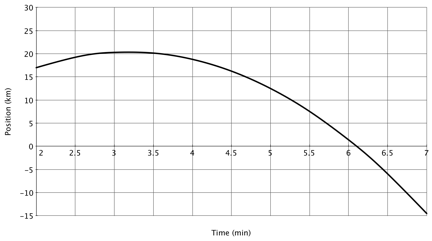
\includegraphics[scale=.5]{/Users/jgates/desktop/latex/pics/xgraph2}
%\end{floatingfigure}
 
{\bf \Large{820.}} A rocket blasts off, traveling with an acceleration of ${4~\tfrac{m}{s^2}}$ upward.  When it is 2000 meters above the ground, its engine shuts off. \bigskip

How much time was required for the rocket to reach the 2000 meter altitude, and how fast was it moving at that moment? \paragraph{}
\noindent
\bigskip 
How fast is the rocket moving when it hits the ground?

%\begin{center}
%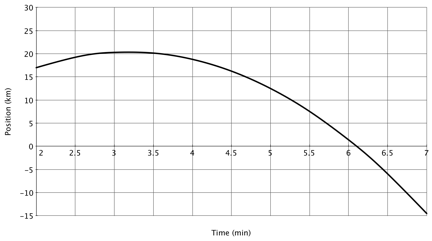
\includegraphics[scale=1]{/Users/jgates/desktop/latex/pics/xgraph2}
%\end{center}

\bigskip \vspace{6mm}% Number 830
% CAPMA Algebra Units 
% Throwing chestnuts - hard
% JG

% Watermark
\AddToShipoutPicture*{\BackgroundPic}

\addtocounter {ProbNum} {1}

%\begin{floatingfigure}[r]{.44\textwidth}
%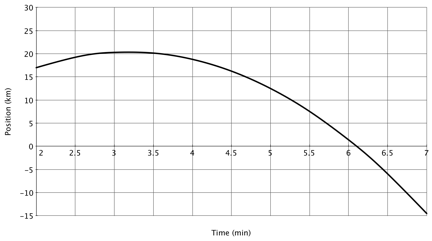
\includegraphics[scale=.5]{/Users/jgates/desktop/latex/pics/xgraph2}
%\end{floatingfigure}
 
{\bf \Large{830.}} While sitting on a tree branch 9 meters above the ground (you're quite a climber!), you drop a chestnut.  When it's halfway to the ground, you throw a second chestnut downward.  \bigskip

What initial speed do you need to give the second chestnut so that it strikes the ground at the same time as the first chestnut?\paragraph{}
\noindent
\vfill

%\begin{center}
%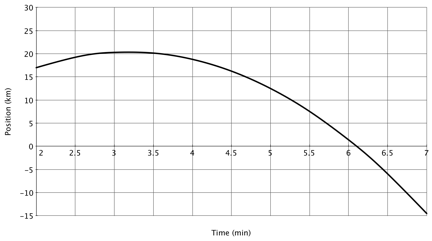
\includegraphics[scale=1]{/Users/jgates/desktop/latex/pics/xgraph2}
%\end{center}


\vspace{6mm}% Number 840
% CAPMA Algebra Units 
% Model rocket - thrust plus freefall, algebraic
% JG

% Watermark
\AddToShipoutPicture*{\BackgroundPic}

\addtocounter {ProbNum} {1}

%\begin{floatingfigure}[r]{.44\textwidth}
%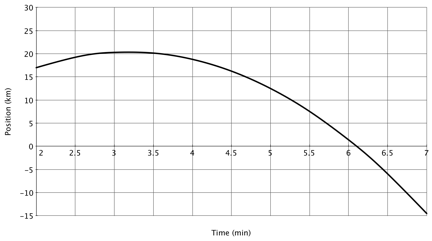
\includegraphics[scale=.5]{/Users/jgates/desktop/latex/pics/xgraph2}
%\end{floatingfigure}
 
{\bf \Large{840.}} A model rocket lifts off and flies with an acceleration of ${12~\tfrac{m}{s^2}}$, until it reaches a height of 26 meters, at which time it continues its flight without any engine thrust.    \bigskip

What maximum speed does the rocket reach?\paragraph{}
\noindent
\vfill

What maximum height does it reach?

\bigskip %\begin{center}
%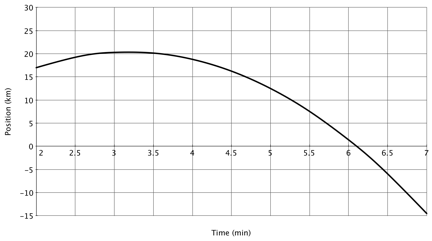
\includegraphics[scale=1]{/Users/jgates/desktop/latex/pics/xgraph2}
%\end{center}


\vspace{6mm}% Number 850
% CAPMA Algebra Units 
% Hot air balloon camera drop
% JG

% Watermark
\AddToShipoutPicture*{\BackgroundPic}

\addtocounter {ProbNum} {1}

%\begin{floatingfigure}[r]{.44\textwidth}
%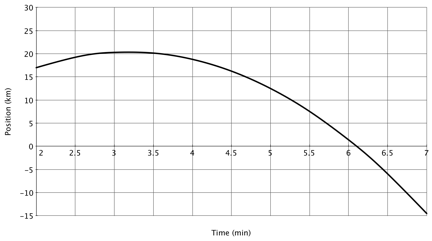
\includegraphics[scale=.5]{/Users/jgates/desktop/latex/pics/xgraph2}
%\end{floatingfigure}
 
{\bf \Large{850.}} A hot-air balloon is 45 meters off of the ground, ascending at a rate of 2 meters per second, when the pilot drops (releases) his camera.  \bigskip

How long will it take to hit the ground?\paragraph{}
\noindent
\vfill


%\begin{center}
%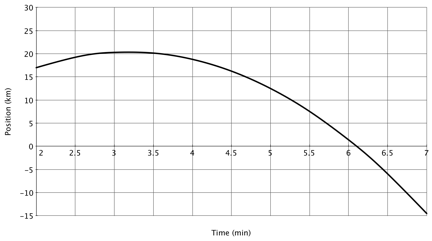
\includegraphics[scale=1]{/Users/jgates/desktop/latex/pics/xgraph2}
%\end{center}


\vspace{6mm}% Number 860
% CAPMA Algebra Units 
% Car skidding to a stop algebraic
% JG

% Watermark
\AddToShipoutPicture*{\BackgroundPic}

\addtocounter {ProbNum} {1}

%\begin{floatingfigure}[r]{.44\textwidth}
%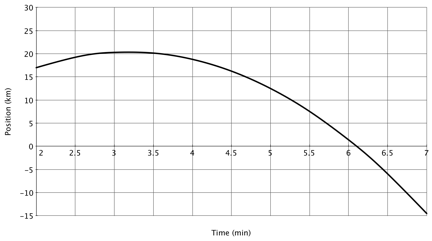
\includegraphics[scale=.5]{/Users/jgates/desktop/latex/pics/xgraph2}
%\end{floatingfigure}
 
{\bf \Large{860.}} A car traveling with a speed of 30 meters per second (a little more than 60 mph) slams on the brakes, coming to a stop after 82 meters (nearly a football field!) of skidding.   \bigskip

How long did this slide take?\paragraph{}
\noindent
\vfill


%\begin{center}
%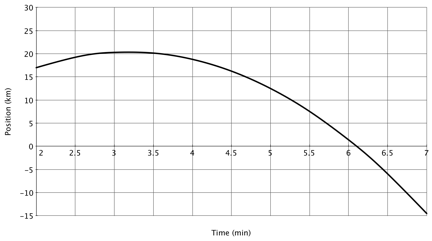
\includegraphics[scale=1]{/Users/jgates/desktop/latex/pics/xgraph2}
%\end{center}


\vspace{6mm}% Number 871
% CAPMA Algebra Units 
% Car skidding to a stop algebraic
% JG

% Watermark
\AddToShipoutPicture*{\BackgroundPic}

\addtocounter {ProbNum} {1}

%\begin{floatingfigure}[r]{.44\textwidth}
%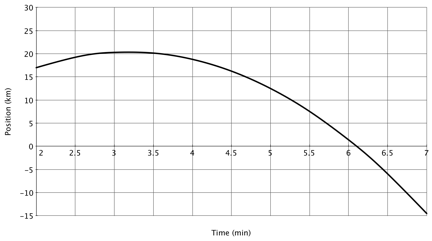
\includegraphics[scale=.5]{/Users/jgates/desktop/latex/pics/xgraph2}
%\end{floatingfigure}
 
{\bf \Large{871.}} A car traveling with a speed of 30 meters per second (a little more than 60 mph) slams on the brakes.  The wheels lock up and the tires skid on the road, providing an acceleration of magnitude ${11~\tfrac{m}{s^2}}$.   \bigskip

How far did the car travel during the slide? Use algebraic methods.\paragraph{}
\noindent
\bigskip 

%\begin{center}
%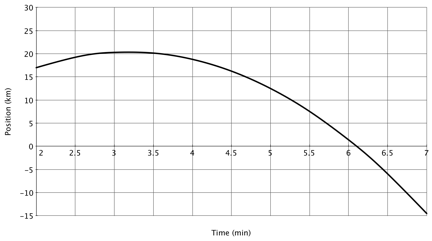
\includegraphics[scale=1]{/Users/jgates/desktop/latex/pics/xgraph2}
%\end{center}


\vspace{6mm}% Number 910
% CAPMA Algebra  Units 
% US Open putt
% JG

% Watermark
\AddToShipoutPicture*{\BackgroundPic}

\addtocounter {ProbNum} {1}

%\begin{floatingfigure}[r]{.44\textwidth}
%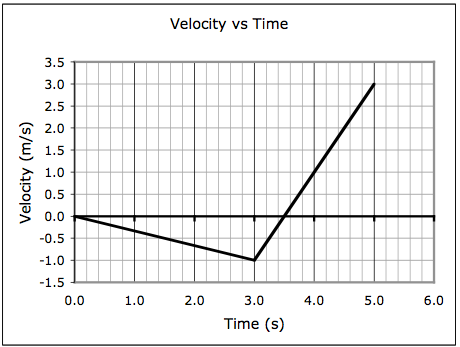
\includegraphics[scale=.54]{/Users/jgates/desktop/latex/pics/vgraph6}
%\end{floatingfigure}
 
{\bf \Large{910.}} In the US Open, you need to make a 7.2 meter putt to win.  You give the ball an initial speed of 4.6 meters per second, but it stops 1.8 meters short of the hole.  (That's OK: you still get a really big check!) \bigskip

If you had hit the ball with the minimum initial speed that would have gotten it into the hole, how long would you have had to wait breathlessly to see if it was going to roll in?
\vfill


%\begin{center}
%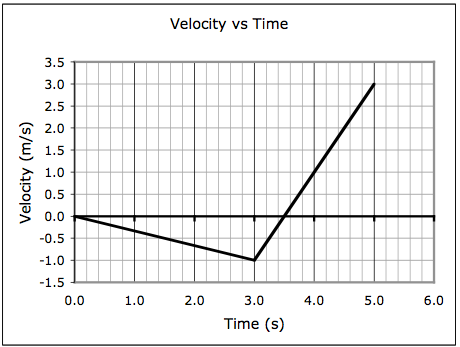
\includegraphics[scale=1]{/Users/jgates/desktop/latex/pics/vgraph6}
%\end{center}


\vspace{6mm}% Number 921
% CAPMA Algebra  Units 
% Rocket upwards - max. v, h? Algebraic
% JG

% Watermark
\AddToShipoutPicture*{\BackgroundPic}

\addtocounter {ProbNum} {1}

%\begin{floatingfigure}[r]{.44\textwidth}
%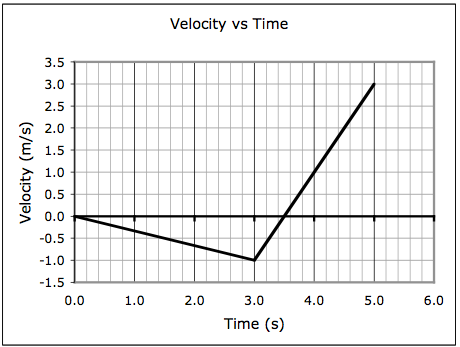
\includegraphics[scale=.54]{/Users/jgates/desktop/latex/pics/vgraph6}
%\end{floatingfigure}
 
{\bf \Large{921.}} A rocket launches and travels upwards with an acceleration of ${4.5~\tfrac{m}{s^2}}$ for 6 seconds; at that point it runs out of fuel and goes into freefall.   \bigskip

Determine the rocket's maximum speed on the upwards trip and amount of time that it will take for it to hit the ground (from launch to impact).  \vfill


%\begin{center}
%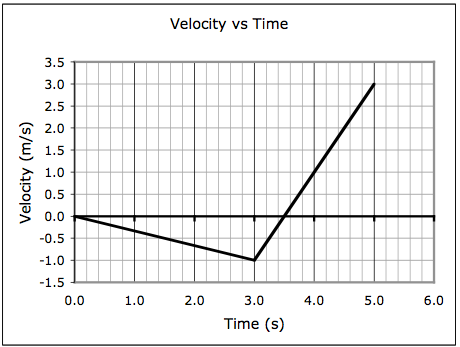
\includegraphics[scale=1]{/Users/jgates/desktop/latex/pics/vgraph6}
%\end{center}


\vspace{6mm}% Number 930
% CAPMA CVPMA Algebra  Units 
% Car driving - CAPM then CVPM, Algebraic
% JG

% Watermark
\AddToShipoutPicture*{\BackgroundPic}

\addtocounter {ProbNum} {1}

%\begin{floatingfigure}[r]{.44\textwidth}
%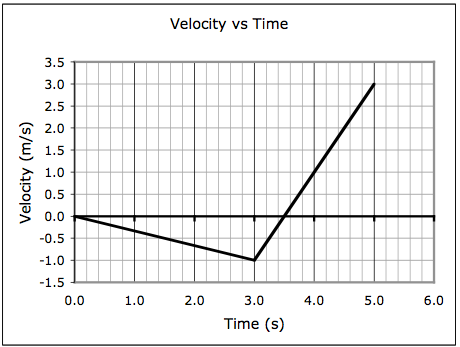
\includegraphics[scale=.54]{/Users/jgates/desktop/latex/pics/vgraph6}
%\end{floatingfigure}
 
{\bf \Large{930.}} A car accelerates from rest to ${25~\tfrac{m}{s}}$ in 4.3 seconds, and then maintains that speed for 10 seconds.    \bigskip

How far has it traveled during this motion?  \vfill


%\begin{center}
%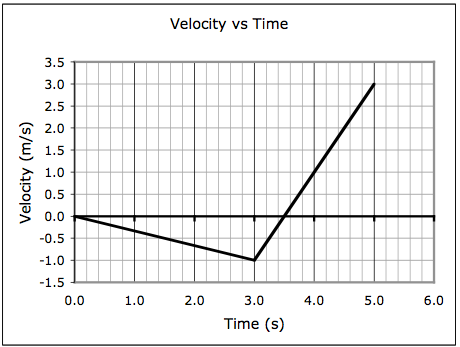
\includegraphics[scale=1]{/Users/jgates/desktop/latex/pics/vgraph6}
%\end{center}


\vspace{6mm}% Number 940
% CAPMA Algebra Units 
% Softball player slide - algebraic
% JG

% Watermark
\AddToShipoutPicture*{\BackgroundPic}

\addtocounter {ProbNum} {1}

%\begin{floatingfigure}[r]{.44\textwidth}
%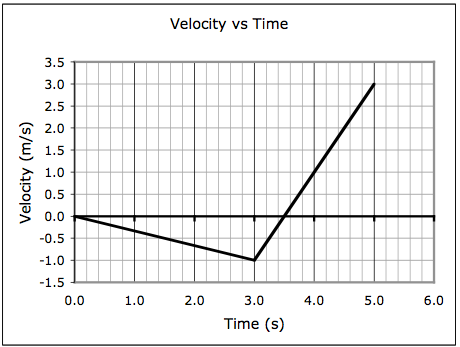
\includegraphics[scale=.54]{/Users/jgates/desktop/latex/pics/vgraph6}
%\end{floatingfigure}
 
{\bf \Large{940.}} A softball player slides into home; as she crosses home plate, she is moving with a speed of ${3~\tfrac{m}{s}}$.  Her slide took .4 seconds and began 1.8 meters from home plate.  \bigskip

What were the magnitude (size) and direction of her acceleration during the slide? \vfill


%\begin{center}
%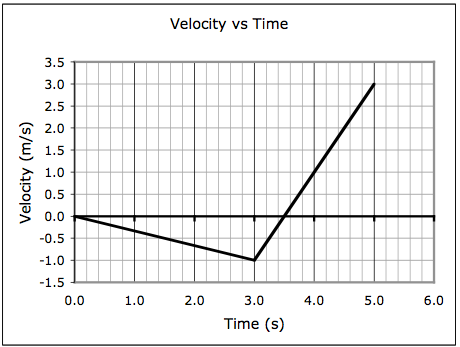
\includegraphics[scale=1]{/Users/jgates/desktop/latex/pics/vgraph6}
%\end{center}


\vspace{6mm}% Number 940
% CAPMA Algebra Units 
% Softball player slide - algebraic
% JG

% Watermark
\AddToShipoutPicture*{\BackgroundPic}

\addtocounter {ProbNum} {1}

%\begin{floatingfigure}[r]{.44\textwidth}
%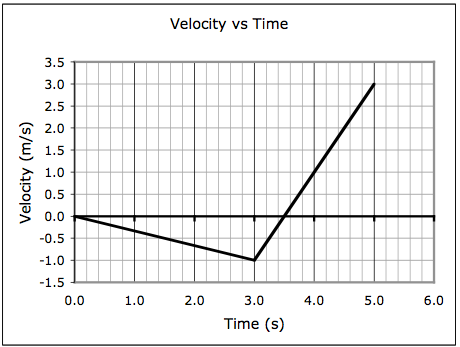
\includegraphics[scale=.54]{/Users/jgates/desktop/latex/pics/vgraph6}
%\end{floatingfigure}
 
{\bf \Large{950.}} A softball player slides into home; as she crosses home plate, she is moving with a speed of ${3~\tfrac{m}{s}}$.  Her slide took .4 seconds and began 1.8 meters from home plate.  \bigskip

What were the magnitude (size) and direction of her acceleration during the slide? \vfill


%\begin{center}
%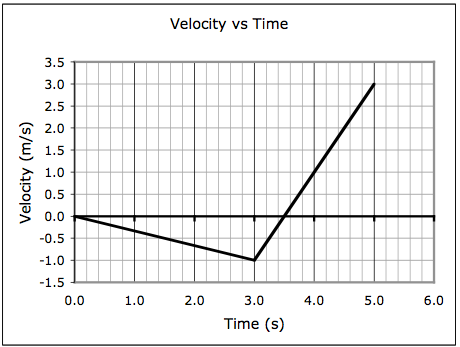
\includegraphics[scale=1]{/Users/jgates/desktop/latex/pics/vgraph6}
%\end{center}


\vspace{6mm}% Number 961
% CAPMA CVPMA Algebra Units 
% Drag racer - CAPM and CVPM - algebraic
% JG

% Watermark
\AddToShipoutPicture*{\BackgroundPic}

\addtocounter {ProbNum} {1}

%\begin{floatingfigure}[r]{.44\textwidth}
%\includegraphics[scale=.54]{/Users/jgates/desktop/latex/pics/vgraph6}
%\end{floatingfigure}
 
{\bf \Large{961.}} A drag racer begins at rest, and accelerates to ${124~\tfrac{m}{s}}$ within 2.2 seconds.  Once at this speed, the racer maintains it through the finish line, which is 400 meters from the start line. \bigskip

How long does it take for the driver to finish the race?
\bigskip 
The car deploys a parachute after crossing the finish line.  The magnitude of the acceleration provided by the air hitting the parachute is ${12~\tfrac{m}{s^2}}$.  How far will the car travel while the parachute is stopping it? 

\bigskip 
What assumptions did you make to solve this problem?  Are they good assumptions?
\bigskip %\begin{center}
%\includegraphics[scale=1]{/Users/jgates/desktop/latex/pics/vgraph6}
%\end{center}


\vspace{6mm}% Number 991
% CAPMA CVPMA Algebra Units 
% Deer stopping, with reaction time - algebraic
% JG

% Watermark
\AddToShipoutPicture*{\BackgroundPic}

\addtocounter {ProbNum} {1}

%\begin{floatingfigure}[r]{.44\textwidth}
%\includegraphics[scale=.95]{/Users/jgates/desktop/latex/pics/agraph1}
%\end{floatingfigure}
 
{\bf \Large{991.}} A car roars down the street, driving ${28~\tfrac{m}{s}}$.  A deer steps into the road 30 meters ahead of the car.  The driver has a .4 second reaction time, after which she slams on the brakes.  The brakes have the ability to stop the car within 1.6 seconds when traveling at this speed (those are pretty great brakes, BTW!).  \bigskip

Two questions: find the car�s acceleration, and�will she stop before hitting the deer?  
\paragraph{}
\noindent
\bigskip 

%\begin{center}
%\includegraphics[scale=.7]{/Users/jgates/desktop/latex/pics/vgraph8}
%\end{center}



\vspace{6mm}% Number 992
% CAPMA Algebra Units 
% Deer stopping, no reaction time - algebraic
% JG

% Watermark
\AddToShipoutPicture*{\BackgroundPic}

\addtocounter {ProbNum} {1}

%\begin{floatingfigure}[r]{.44\textwidth}
%\includegraphics[scale=.95]{/Users/jgates/desktop/latex/pics/agraph1}
%\end{floatingfigure}
 
{\bf \Large{992.}} A truck drives down a dark highway, driving ${34~\tfrac{m}{s}}$.  A deer steps into the road 30 meters ahead of the car.  The driver has a .3 second reaction time, after which he slams on the brakes.  The brakes have the ability to stop the car within 1.8 seconds when traveling at this speed.  \bigskip

Will he stop before hitting the deer?  
\paragraph{}
\noindent
\bigskip 

%\begin{center}
%\includegraphics[scale=.7]{/Users/jgates/desktop/latex/pics/vgraph8}
%\end{center}



\vspace{6mm}\end{document}